\documentclass{article}

\usepackage{tikz}

\usetikzlibrary{shapes.geometric,calc}

\begin{document}
	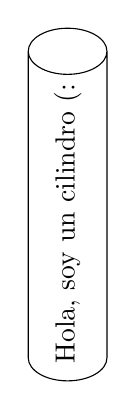
\begin{tikzpicture}
		\node [cylinder, rotate=90, draw, minimum height=2cm,
		minimum width=1cm] (c) {Hola, soy un cilindro (:} ;
	\end{tikzpicture}
\hspace{2cm}
% orientaci'on
%   (y,z,x)
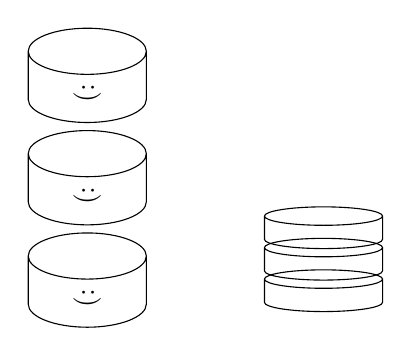
\begin{tikzpicture}
	\tikzset{every node/.style={cylinder, rotate=90, draw}}

	\node [minimum width=1.5cm] at (0,0,0)		{(:};
	\node [minimum width=1.5cm] at (0,1.3,0) 	{(:};
	\node [minimum width=1.5cm] at (0,2.6,0) 	{(:};

	\node [minimum width=1.5cm] at (3,0,0)   	{};
	\node [minimum width=1.5cm] at (3,.4,0) 	{};
	\node [minimum width=1.5cm] at (3,.8,0) 	{};
\end{tikzpicture}

\def\ficheraZoom{
  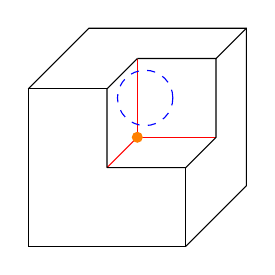
\begin{tikzpicture}[scale=1]
    \coordinate (a0) at (0,0,0);
    \coordinate (a1) at (1,0,0);
    \coordinate (a2) at (0,1,0);
    \coordinate (a3) at (0,0,1);
    \draw[red] (a1) -- (a0);
    \draw[red] (a0) -- (a2);
    \draw[red] (a3) -- (a0);
    \draw (a2) -- ($(a1)+(a2)$) -- (a1) -- ($(a1) + (a3)$) -- (a3);
    \draw (a2) -- ($(a3)+(a2)$) -- (a3);
    \draw ($(a3)+(a2)$) -- ($(a3)+(a2)-(a1)$) -- ($(a3)-(a2)-(a1)$)
      -- ($(a1)-(a2)+(a3)$) -- ($(a1)+(a3)$);
    \draw ($(a1)-(a2)+(a3)$) -- ($(a1)-(a2)-(a3)$) -- ($(a1)+(a2)-(a3)$)
      -- ($(a2)-(a1)-(a3)$) -- ($(a2)-(a1)+(a3)$);
    \draw ($(a1)+(a2)-(a3)$) -- ($(a1)+(a2)$);
    \fill[orange] (a0) circle (2pt);
    \draw[dashed,blue] (0.1,.5,0) circle (10pt);
  \end{tikzpicture}
}

\ficheraZoom

\end{document}